
\documentclass[12pt]{article} 
\usepackage[utf8]{inputenc}
\usepackage[slovak]{babel}
\usepackage[hidelinks,unicode = true]{hyperref}
\usepackage{outline}
\usepackage{graphicx}
%\usepackage{biblatex}
%\addbibresource{literatura.bib}
\usepackage{cite}
\usepackage{caption}
\setcounter{secnumdepth}{3}
\setcounter{tocdepth}{3}

%===========================================================================
\begin{document}           % Konec preambule a zároveň začátek vlastního textu
\begin{titlepage}
\centering
\Large \textbf{České vysoké učení technické v Praze }\\ Fakulta stavební
\vspace{2cm}

\begin{figure}[h!] %logoCVUT
\centering
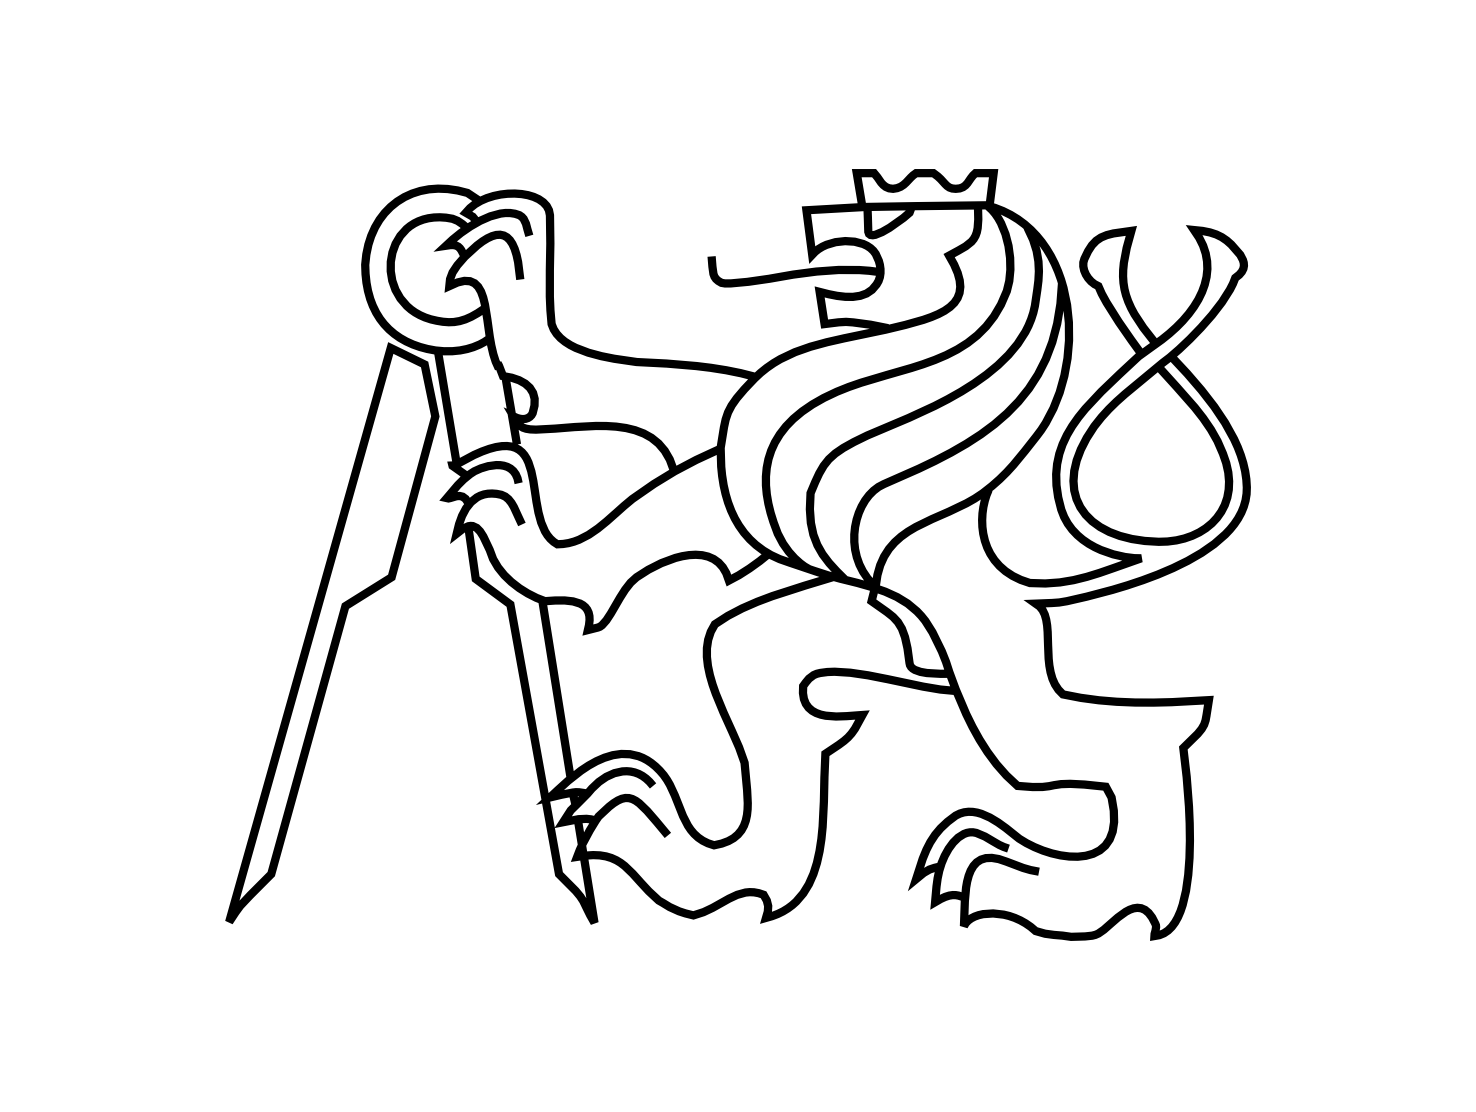
\includegraphics[width=7cm]{./img/cvut.png}
\end{figure}
 
\Large \textbf{155ADKG Algoritmy v digitální kartografii}
\vspace{1cm}

\LARGE  \textbf{Geometrické vyhľadávanie bodu}
\vspace{3cm}

\Large Bc. Lukáš Kettner Bc. Martin Hulín \\ 23.10.2019

 \thispagestyle{empty} %neočísluje první stránku
\end{titlepage}

\tableofcontents    % vytváří  Obsah 
\newpage %začne na nové stránce
%------------------------------------------------------------------------
\section{Zadanie}
Vytvorte aplikáciu s grafickým rozhraním, ktorá určí polohu bodu voči polygónovej mape. Vstup do aplikácie : súvislá polygónová mapa n polygónov \{P1, …, Pn\} , analyzovaný bod q. Výstup aplikácie : Pi, q $\in$ Pi.

Nad polygónovou mapou implementujte nasledujúce algoritmy pre geometrické vyhľadávanie:

\begin{itemize}
\item Ray Crossing Algorithm (varianta s posunom ťažiska polygónu).
\item Winding Number Algorithm	
\end{itemize}
		
Nájdený polygón obsahujúci zadaný bod q graficky zvýraznite vhodným spôsobom. Grafické rozhranie vytvorte s použitím frameworku Qt. Pre generovanie nekonvexných polygónov môžete navrhnúť vlastný algoritmus alebo použiť existujúce geografické dáta. Polygóny budú načítane z textového súboru vo Vami zvolenom formáte. Pre dátovú reprezentáciu jednotlivých modelov použite špagetový model.

\subsection{Bonusové úlohy}
V rámci úlohy sú vypracované tieto bonusové úlohy

\begin{itemize}
\item Ošetrenie singulárneho prípadu pri Winding Number Algorithm. \textit{+2b}
\item Ošetrenie singulárneho prípadu pri oboch algoritmoch. \textit{+2b}
\item Zvýraznenie všetkých polygónov pre oba uvedené singulárne prípady. \textit{+2b}
\item Algoritmus pre automatické generovanie nekonvexných polygónov. \textit{+5b}
\end{itemize}
%------------------------------------------------------------------------

\section{Popis a rozbor problému}
 Problematikou úlohy je určenie vzájomného vzťahu polohy medzi bodom a danou oblasťou. Oblasť je tvorená polygónovou mapou. Pre bod sme zvolili označenie q. Následne analýzou pomocou dvoch typov algoritmov rozhodujeme o vzájomnej polohe bodu a polygónu.
Varianty výsledkov analýzy :

\begin{itemize}
\item bod q leží vnútri polygónu.
\item bod q leží mimo polygónu.
\item bod q leží na hrane polygónu.
\item bod q je totožný s vrcholom polygónu.
\end{itemize}

Pre učenie polohy bodu voči polygónom boli použité algoritmy Ray Crossing Algorithm a Winding Number Algorithm.
%------------------------------------------------------------------------

\section {Popis použitých algoritmov}
\subsection {Ray Crossing Algorithm}
Ray Crossing Algorithm je takzvaný lúčový algoritmus. Z bodu q, ktorého polohu určujeme, vedieme polopriamku a určíme počet priesečníkov s hranami polygónu. Priesečník priamky s hranami polygónu P označíme k. Potom platí :
\begin{enumerate}
\item Ak k je nepárne – bod q patrí polygónu P (q  $\in$ P).
\item Ak k je párne – bod q nepatrí polygónu P(q  $\notin$ P).
\end{enumerate}

\begin{center}
   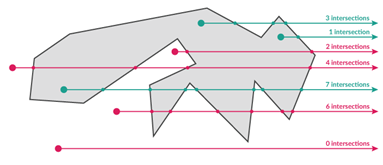
\includegraphics[width=10cm]{./img/ray_algo.png}
   \captionof{figure}{Ray Crossing Algorithm \cite{introWherewolf}}
\end{center}

\subsubsection {Problematické situácie}
Problematickou situáciou je singularita. K singularite dôjde ak bod leží na hrane polygónu alebo je totožný s vrcholom polygónu. V takomto prípade je počet priesečníkov s hranou polygónu párny, aj napriek tomu, že bod q leží vnútri polygónu.

Ošetrenie singularity sa vykoná zavedením miestneho súradnicového systému.
\begin{enumerate}
\item Počiatok sústavy je vložený do bodu q
\item Os x' je rovnobežná s osou x
\item Os y' je kolmá na os x'
\end{enumerate}	
Riešenie sa v takomto prípade týka len takých hrán polygónu, ktorých jeden bod leží nad osou x' a druhý pod osou x' . Prípad kedy je bod q totožný s vrcholom polygónu alebo leží na hrane polygónu sa ošetrí pomocou určenia dĺžky hrany polygónu a následne súčtom vzdialeností medzi bodom q a vrcholmi hrany. Pokiaľ sú tieto vzdialenosti identické, bod leží na hrane polygónu alebo je totožný s jeho vrcholom.

\subsubsection {Implementácia metódy}
\begin{enumerate}
\item Inicializácia k = 0.
\item Určenie veľkosti polygónu int n =pol.size()
\item Redukcia súradníc X a Y na bod q $\to$ x', y'.
\item Určenie veľkosti polygónu int n =pol.size()
\item Cyklus for pre všetky body polygónu
\item Podmienka v cykle pre započítanie priesečníkov
\item[] $if(y_i' >0) \&\& (y_{i-1}' \leq 0) \|\| (y_{i-1}' > 0) \&\& (y_i' \leq 0)$

\begin{itemize}
\item[] $x_m'=(x_i'y_{i-1}'-x_{i-1}'y_i')/(y_i'-y_{i-1}')$
\item[] $if(x_m'>0), k = k+1$
\end{itemize}

\item if(k \% 2) $\neq 0$ $potom$ $q \in P$.
\item inak q $\notin$ P
\end{enumerate}

\subsection {Winding Number Algorithm}

Metóda Winding Number je používaná pre určenie pozície bodu voči nekonvexným mnohouholníkom. Algoritmus si môžeme predstaviť ako nasledujúcu situáciu. Postavíme sa na určovaný bod a otáčame sa postupne ku každému vrcholu polygónu. Pokiaľ sa otáčame po smere hodinových ručičiek, uhol sčítame, v opačnom prípade odčítame. Pokiaľ je výsledný uhol rovný 2$\pi$, bod na ktorom stojíme leží vnútri polygónu. Pri tejto metóde je potrebné určiť Winding Number $\Omega$. $\Omega$ je rovné sume rotácií $\omega$ proti smeru hodinových ručičiek, ktoré prievodič opíše nad všetkými bodmi $\Omega = \sum_{i=1}^{n}*\omega_i$. Určíme uhly $\omega_i(p_i,q,p_{i+1})$. \\[2pt]

$\cos \omega_i = \frac{\vec u_i *\vec v_1}{\parallel \vec u_i \parallel*\parallel \vec v_i \parallel}; \vec u_i = (q, p_i), \vec v_i = (q, p_{i+1})$ \\[2pt]

Pokiaľ je uhol orientovaný v sme re hodinových ručičiek, nadobúda kladné znamienko. V protismere hodinových ručičiek záporné znamienko. Podľa sumy všetkých uhlov určíme polohu bodu q.\\[2pt]

Ak je $\sum \omega_i = $
\begin{enumerate}
\item 360$^\circ$ bod q $\in$ Pj
\item 0$^\circ$ bod q $\notin$ P
\item inak bod leží na hranici polygónu alebo vo vrchole polygónu
\end{enumerate}

\begin{center}
   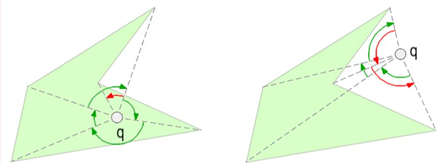
\includegraphics[width=10cm]{./img/windin_alg.png}
   \captionof{figure}{Winding Number Algorithm \cite{geomVyhl}}
\end{center}	

\subsubsection{Problematické situácie}
K singulárnym prípadom dôjde pri Winding Algoritmu ak je poloha určovaného bodu zhodná s polohou vrcholu polygónu. Je potreba ošetriť blízkosť hodnôt.
$\sum \omega \neq360^\circ \omega \neq 0^\circ q \in \sigma_{pi}$

\subsubsection{Implementácia metódy}
\begin{enumerate}
\item Inicializácia $\omega = 0$, tolerancia $\epsilon$ 
\item Určenie veľkosti polygónu int n =pol.size()
\item Cyklus for - prechádzame všetky body polygónu
\item Určenie veľkosti uhlu $\omega_i = \angle p_i,p_{i+1} $
\item[] Podmienka if,pokiaľ bod vľavo $\omega = \omega + \omega_i$; else $\omega = \omega - \omega_i$
\item $if(|\omega-2\pi|< \epsilon)$  tak $q \in P$
\item else $q \notin P$
\end{enumerate}
%------------------------------------------------------------------------

\section{Vstupné dáta}
\subsection{Polygónová mapa}
Polygónovú mapu do našej aplikácie importujeme pomocou textového súboru *.txt, ktorý obsahuje :

\begin{itemize}
\itemsep0em
\item počet polygónov
\item počet bodov v prvom polygóne, súradnice x a y oddelené medzerou
\item počet bodov v druhom polygóne, súradnice x a y oddelené medzerou
\item počet bodov v treťom polygóne, súradnice x a y oddelené medzerou
\item počet bodov v štvrtom polygóne, súradnice x a y oddelené medzerou
\item počet bodov v piatom polygóne, súradnice x a y oddelené medzerou
\end{itemize}

\begin{center}
   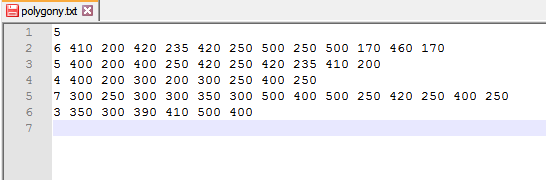
\includegraphics[width=10cm]{./img/txt_subor.png}
   \captionof{figure}{Textový formát polygónovej mapy}
\end{center}

\subsection{Bod q}
Súradnice bodu q sa do aplikácie zadávajú kliknutím myšou.
%------------------------------------------------------------------------

\section{Ukážka vytvorenej aplikácie}
Načítanie polygónovej mapy sa uskutoční pomocou tlačidla Import polygon. Po zadaní *.txt súboru sa objaví dialógové okno, ktoré oznamuje počet nahratých polygónov. Po stlačení tlačidla „OK“ sa polygóny vykreslia.

\begin{center}
   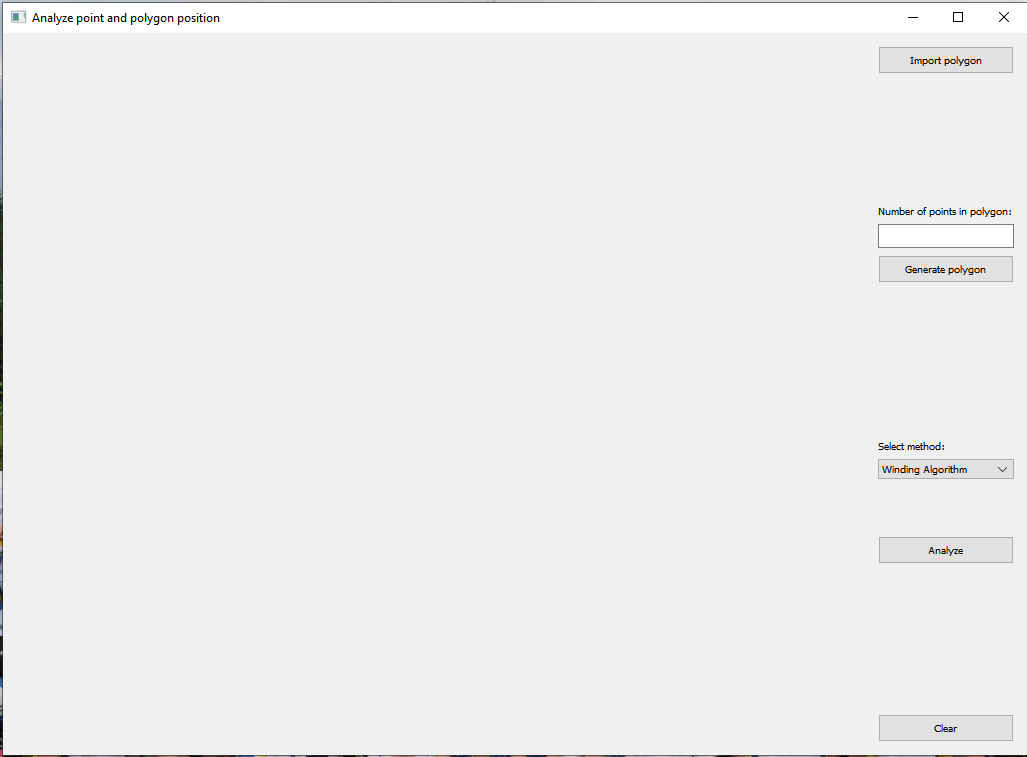
\includegraphics[width=9cm]{./img/import.png}
   \captionof{figure}{Uvodné okno}
\end{center}

\begin{center}
   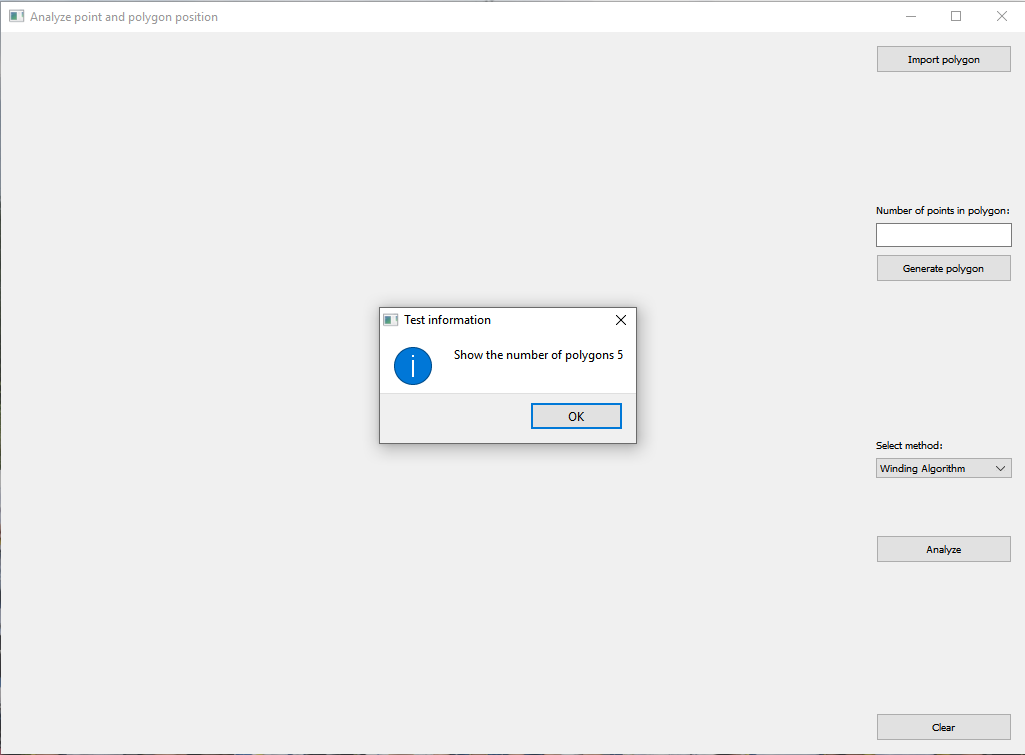
\includegraphics[width=9cm]{./img/import2.png}
   \captionof{figure}{Informace o počtě načítaných polygónov}
\end{center}

\begin{center}
   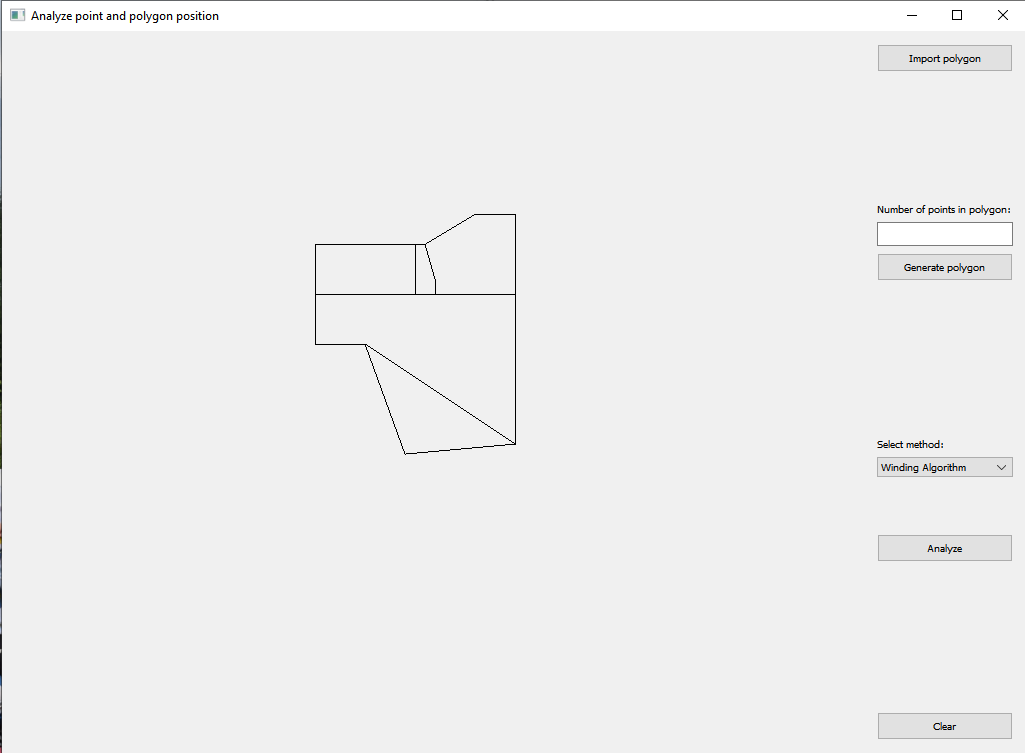
\includegraphics[width=9cm]{./img/import3.png}
   \captionof{figure}{Zobrazenie polygónovej mapy}
\end{center}

Následne kliknutím myšou do vykreslovacieho plátna zadáme polohu bodu q. Následne po stlačení tlačidla Analyze sa vykoná analýza polohy bodu q voči polygónovej mape.  

V prípade, že dôjde k neúspešnému nahratiu polygónovej mapy zobrazí sa varovné okno s varovnou hláškou.

\begin{center}
   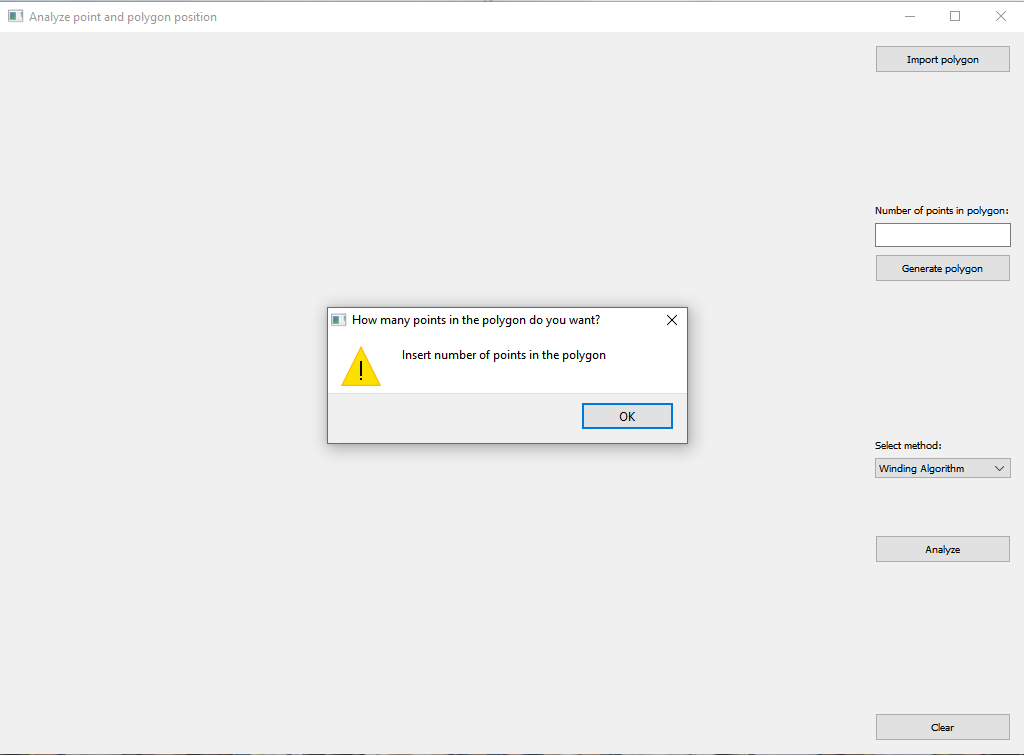
\includegraphics[width=9cm]{./img/warning.png}
   \captionof{figure}{Neúspešné načítanie polygónovej mapy - varovné okno}
\end{center}

\subsection{Generování bodů}
Aplikácia umožňuje generovanie nekonvexného polygónu. Vstupom pre toto generovanie je požadovaný počet bodov v generovanom polygóne.

Generovanie je prevádzané pomocou $std::random\_device$. Použili sme generátor $std::mt19937$(A Mersenne Twister pseudo-random generator of 32-bit numbers). Pre súradnicu x boli hodnoty generované z rozsahu 100 až 700 a pre súradnicu y v  rozsahu 50 až 650 pomocou $std::uniform\_int\_distribution<>$.

\begin{center}
   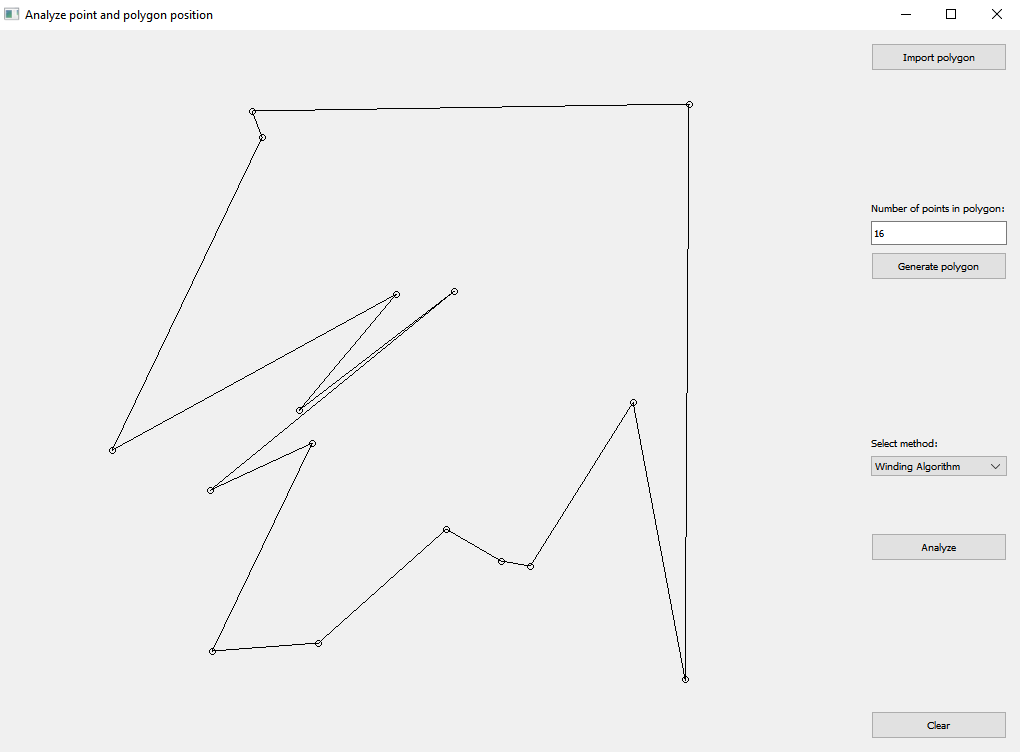
\includegraphics[width=10cm]{./img/generate.png}
   \captionof{figure}{Ukážka vygenerovaného polygonu s 16 bodmi}
\end{center}
%-------------------------------------------------------------------------

\section{Výsledok analýzy}
V grafickom rozhraní aplikácie sa po vykonaní analýzy zobrazí výsledok analýzy. Pokiaľ bod leží v polygóne, vysvieti a vyšráfuje sa polygón obsahujúci bod q. Pokiaľ bod leží v spoločnom vrchole viacerých polygónov vysvietia a vyšráfujú sa všetky polygóny pre ktoré je daný vrchol spoločný. Pokiaľ bod leží mimo polygónu v grafickom rozhraní aplikácie nenastane žiadna zmena. O polohe bodu takisto invormuje hláška vypísaná v label pod tlačidlom Analyze.

\begin{center}
   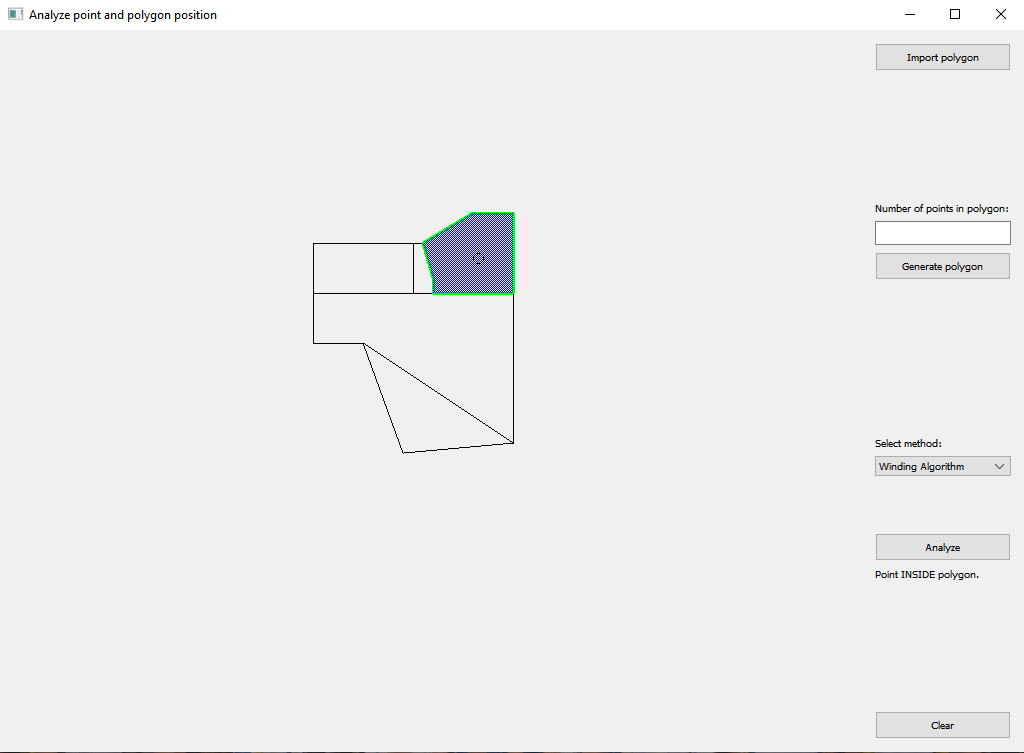
\includegraphics[width=9cm]{./img/bod_v_polygone.png}
   \captionof{figure}{Bod q vnútri polygónu}
\end{center}

%\begin{center}
%  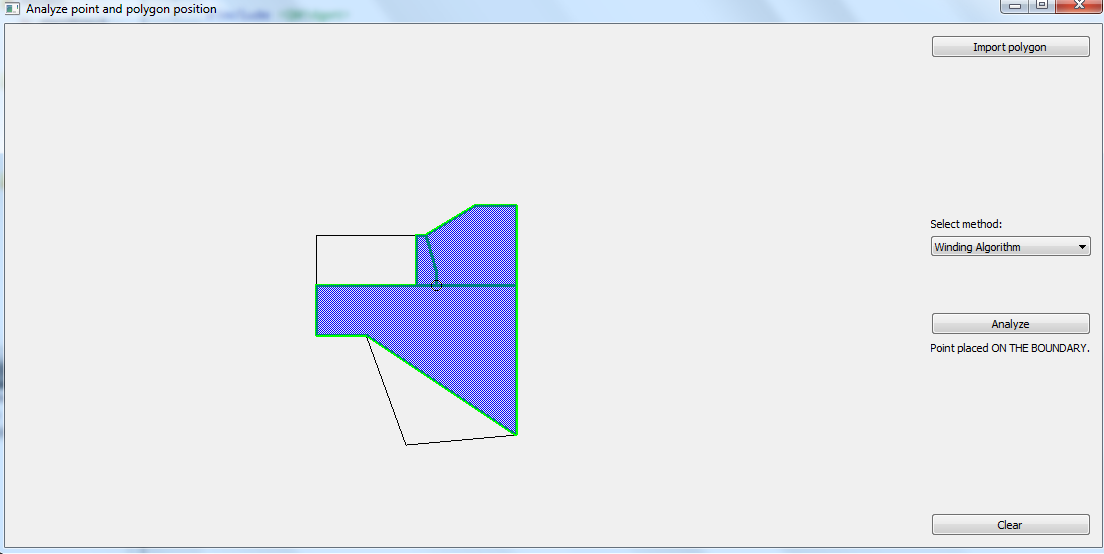
\includegraphics[width=10cm]{./img/bod_na_vrchole.png}
%   \captionof{figure}{Bod q v spoločnom vrchole viacerých polygónov}
%\end{center}

\begin{center}
   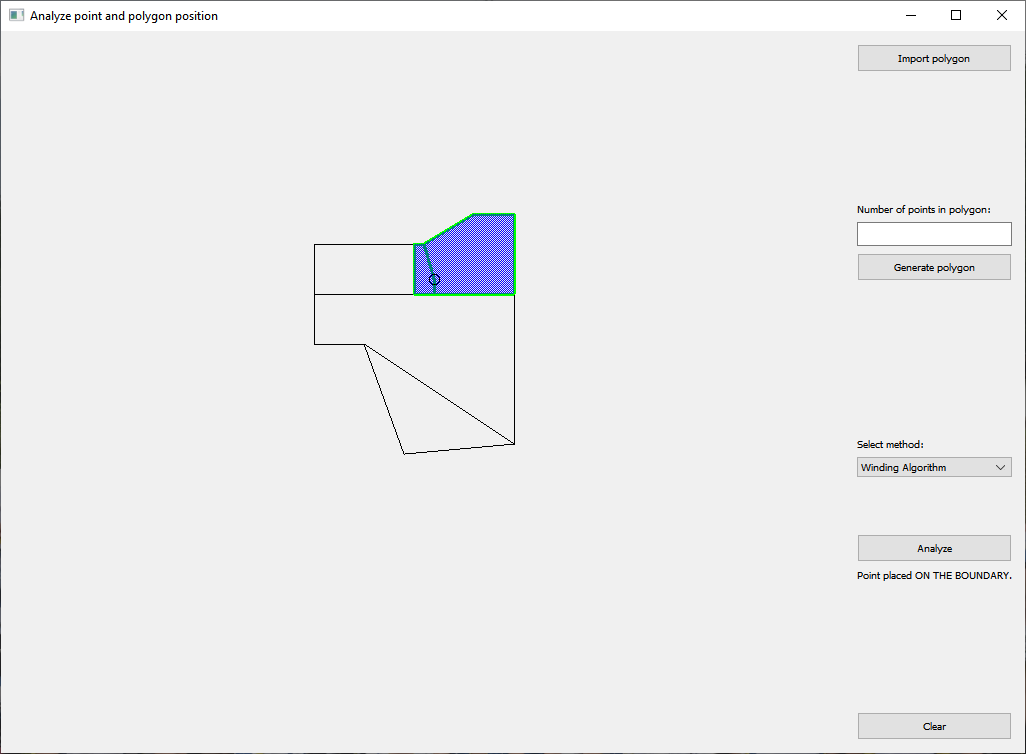
\includegraphics[width=9cm]{./img/na_hrane.png}
   \captionof{figure}{Bod q na hrane}
\end{center}

\begin{center}
   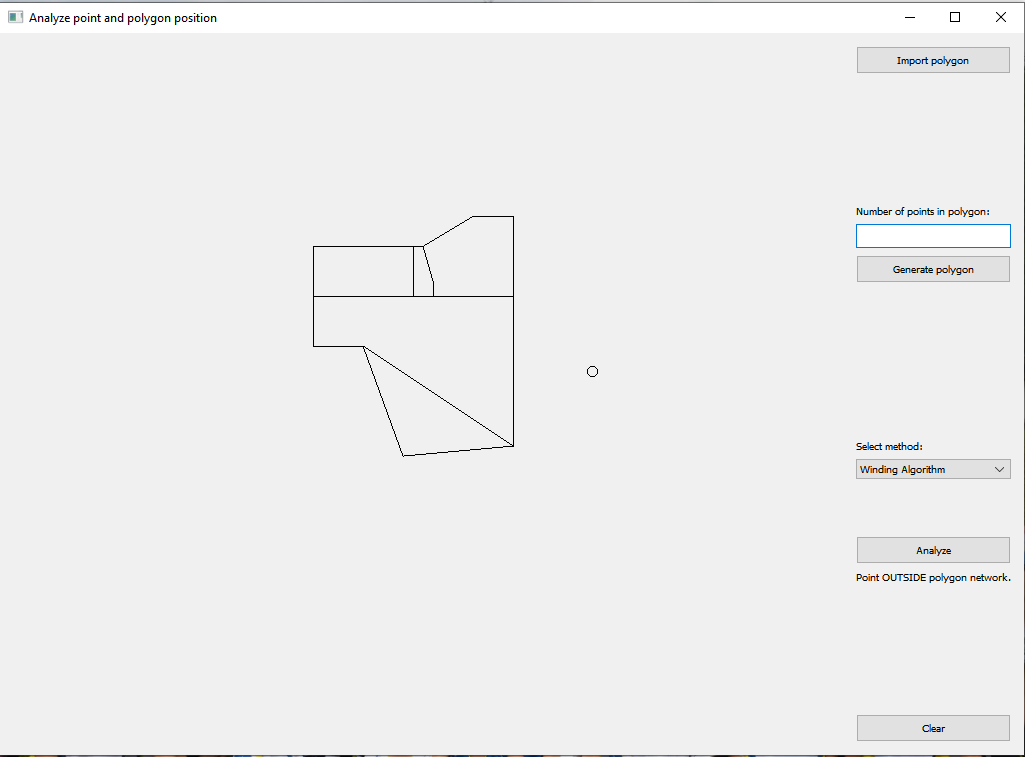
\includegraphics[width=9cm]{./img/mimo.png}
   \captionof{figure}{Bod q mimo polygónu}
\end{center}
%-------------------------------------------------------------------------

\section{Dokumentácia}
\subsection{Trieda Algorithms}
Triedu Algorithms sme použili pre deklarovanie funkcií pre výpočtové algoritmy určenia polohy bodu voči polygónu a pre deklaráciu ich pomocných metód.

\subsubsection{Metódy}

\begin{enumerate}
\item[] \underline{positionPointPolygonRayCrossing}
\begin{itemize}
\item slúži k určeniu polohy bodu prostredníctvom Ray Crossing algoritmu.Návratový typ je integer.

\item na vstupe má : QPoint q -- bod ktorého polohu určujeme, std$::$vector$<$QPoint$>$ pol -- polygon, voči ktorému určujeme polohu bodu q  

\item výstupom je hodnota :
\item[] -1 – bod sa nachádza na hranici alebo vo vrchole polygónu
\item[] 0 – bod sa nachádza mimo polygón
\item[] 1 – bod sa nachádza vnútri polygónu

\end{itemize}
\item[] \underline{positionPointPolygonWinding}
\begin{itemize}
\item slúži k určeniu polohy bodu prostredníctvom Winding Number algoritmu. Jej návratový typ je integer.
\item na vstupe má : QPoint q – bod ktorého polohu určujeme, std$::$vector$<$QPoint$>$ pol – polygon, voči ktorému určujeme polohu bodu q
\item výstupom je hodnota :
\item[] -1 – bod sa nachádza na hranici alebo vo vrchole polygónu
\item[] 0 – bod sa nachádza mimo polygón
\item[] 1 – bod sa nachádza vnútri polygónu
\end{itemize}

\item[] \underline{getAngle2Vectors}
\begin{itemize}
\item je pomocnou metódou pre metódu positionPointPolygonWinding. Slúži k určeniu uhlu medzi dvoma priamkami. Jej návratovou hodnotou je double
\item na vstupe má : súradnice bodov $p_1, p_2, p_3, p_4$ určujúcich prvú a druhú priamku
\item výstupom je hodnota uhlu medzi priamkami 
\end{itemize}

\item[] \underline{getPointLinePosition}
\begin{itemize}
\item je pomocnou metódou pre metódu positionPointPolygonWinding. Slúži na určenie polohy bodu voči priamke. Jej návratovou hodnotou je integer.
\item na vstupe má : súradnice určovaného bodu q , súradnice bodov priamky $p_1$ $p_2$
\item na výstupe hodnoty :
\item[] -1 – bod sa nachádza na priamke
\item[] 0 – bod sa nachádza vpravo od priamky
\item[] 1 – bod sa nachádza vľavo od priamky
\end{itemize}
\item[] \underline{polGen}
\begin{itemize}
\item náhodne generuje polygón s daným počtom bodov. V šúčstnom stave len jeden polygón.
\item Body polygónu se generované v rozsahu 100 - 700 pre x-ovú súradnicu, 50 - 650 pre y-onovú súradnicu.
\item Vstupom je zadaný počet bodov od užívateľa prostredníctvom widget lineEdit.
\end{itemize}
\item[] \underline{GrahamScan}
\begin{itemize}
\item opravuje poradie vstupných bodov podľa veľkosti uhlu omega, tak aby bolo možné zostaviť nekonvený polygón s využitím Graham Scan algoritmu pre tvorbu nekonvexnej obálky.
\end{itemize}
\end{enumerate}

\subsection{Trieda Draw}
Trieda Draw slúži ku grafickému vykresleniu bodu q a polygónovej mapy.

\subsubsection{Členské premenné}

\begin{enumerate}
\item[] \underline{QPoint q}
\begin{itemize}
\item súradnice bodu, ktorého polohu zisťujeme. Východiskové hodnoty sú nastavené v konštruktore. Hodnoty súradníc určovaného bodu sa menia stlačením tlačidla myši na vykreslovacom plátne..
\end{itemize}
\item[] \underline{std$::$vector$<$stdvector$<$QPoint$>>$ polygons}
\begin{itemize}
\item vektor obsahujúci body jednotlivých polygónov
\end{itemize}
\item[] \underline{std$::$vector$<$int$>$ analyze\_results\_by\_polygons}
\begin{itemize}
\item vektor v ktorom sú uložené výsledky analýzy
\end{itemize}
\item[] \underline{std$::$vector$<$QPoint$>$ generated\_points}
\begin{itemize}
\item vektor uloženými vygenerovanými body pro tvorbu generovaného polygonu
\end{itemize}
\end{enumerate}

\subsubsection{Metódy}
\begin{enumerate}
\item[] \underline{paintEvent}
\begin{itemize}
\item slúži k vykresleniu zisťovaného bodu, vykresleniu importu polygónovej mapy a k vyfarbeniu polygónov ktorým náleží určovaný bod q. Návratovým typom je void.
\end{itemize}
\item[] \underline{void mousePressEvent}
\begin{itemize}
\item slúži k vykresleniu bodu q stlačením tlačidla myši, v okamihu stlačenia tlačidla na myši sa uložia súradnice bodu q. Návratovým typom je void.
\end{itemize}
\item[] \underline{void clearCanvas}
\begin{itemize}
\item slúži k vymazaniu obsahu vykreslovacieho plátna. Návratovým typom je void.
\end{itemize}
\item[] \underline{void importPolygon}
\begin{itemize}
\item metóda slúži k importu polygónovej mapy z textového súboru *.txt, ich uloženiu do zoznamu polygónov polygons. Vstupom je cesta k súboru. Výstupom je správa obsahujúca počet nahratých polygónov.etóda slúži k importu polygónovej mapy z textového súboru *.txt, ich uloženiu do zoznamu polygónov polygons. Vstupom je cesta k súboru. Výstupom je správa obsahujúca počet nahratých polygónov.
\end{itemize}
\item[] \underline{int getNumberOfPolygons}
\begin{itemize}
\item slúži k určeniu počtu polygónov v Canvase. Návratový typ je integer.
\end{itemize}
\item[] \underline{void generatePoints}
\begin{itemize}
\item pristupuje k členskej premennej generated\_points a vkládá do nej vygenerované a Graham Scan algoritmom zpracované (zoradené) body.
\end{itemize}
\end{enumerate}

\subsection{Trieda Widget}
Tieda Widget obashuje metódy ktoré sú odkazom na sloty umožňujúce vykonávať príkazy z grafického rozhrania aplikácie. Nemajú žiadne vstupné hodnoty, návratovým typom je void.

\subsubsection{Metódy}
\begin{enumerate}
\item[] \underline{on\_clearButton\_clicked}
\begin{itemize}
\item tlačidlo Clear, vyčistí grafické okno Canvasu
\end{itemize}
\item[] \underline{on\_analyzeButton\_clicked}
\begin{itemize}
\item tlačidlo Analyze. Po jeho stlačení sa vykoná analýza polohy bodu q voči polygónovej mape.
\end{itemize}
\item[] \underline{on\_importPolygonButton\_clicked}
\begin{itemize}
\item tlačidlo Import polygon. Zobrazí sa dialógové okno v ktorom je možné vybrať textový súbor obsahujúci polygónovú mapu. V prípade úspešného nahratia polygónovej mapy za zobrazí dialógové okno s počtom nahratých polygónov. V prípade nesprávneho importu sa zobrazí varovné okno.
\end{itemize}
\item[] \underline{showResultOfAnalysis}
\begin{itemize}
\item pomocou tejto metódy vypisujeme výsledkok analýzy na label v grafickom okne. Vstupom je výsledok analýzy pre jeden polygón a premenná show result, ktorá je typu bool.
\end{itemize}
\end{enumerate}

\subsection{Trieda SortByY}
\begin{itemize}
\item Triedi body vo vektore podľa veľkosti y-onovej súradnice každého bohu. 
\end{itemize}
\subsection{Trieda SortByOmega}
\begin{itemize}
\item Triedi body vo vektore podľa veľkosti uhlu omega. Uhol omega je uhol od rovnobežky daným bodom, najčaštejšie pivotom s minimálnou alebo maximálnou súradnicou. V našom prípade sa jedná o bod s najmenšou y-onovou súradnicou.
\end{itemize}
%-------------------------------------------------------------------------

\section{Záver}
V priebehu vypracovania úlohy sme narazili na množstvo problémov, ktoré sme úspešne dokázali vyriešiť a tým sme obohatili naše vedomosti v oblasti programovania.

Veľké problémy nám spôsobilo správne kódovanie textového súboru. Obsah súboru nebolo možné dlho načítať, s riešením sme strávili niekoľko hodín. Avšak podarilo sa nám tento problém vyriešiť, vykonali sme zmenu kódovania na UTF-8 s BOM (byte order mark).

Výsledkom je funkčná aplikácia, ktorá umožňuje analyzovať polohu bodu voči polygónu z polygónovej mapy. V prípade, vylepšenia aplikácie by bolo zaujímavé implementovať možnosť nahrania *.shp súboru. V takej situácii by bolo potrebné vyriešiť vhodný vstupný formát súboru *.shp. Ďalším možným vylepšením je implementácia algoritmu pre automatické generovanie nekonvexných polygónov. Túto bonusovú úlohu sme z časových dôvodov do našej aplikácie nezakomponovali. Pokúsili sme sa pridať možnosť generovania jedného polygónu. Generovanie je funkčné pre 16 bodov. Pri 17tom bode nastáva nevyriešený problém, znehodnocujúci ďalšie generovanie.

Bohužiaľ po implementování generovania nekonvexného polygónu nastal problém pri analýze pomocou Ray Crossing algoritmu. Túto chybu se nám bohužiaľ aj napriek veľkej snahe a maximálnemu nasadeniu nepodarilo doposiaľ odtraniť a zostáva jedným z cieľov vylepšenia do budúcna.

%-------------------------------------------------------------------------
\nocite{*}
%\printbibliography
\bibliographystyle{plain}
\bibliography{literatura}{}
%-------------------------------------------------------------------------
    
\end{document}             % Konec dokumentu.
